\documentclass[times, utf8, zavrsni]{fer}
\usepackage[titletoc]{appendix}
\usepackage{booktabs}
\usepackage{graphicx}
\usepackage[]{algorithm2e}
\usepackage{caption}
\usepackage{multirow}
\usepackage{listings}
\usepackage{xcolor}
\usepackage{textcomp}
\definecolor{listinggray}{gray}{0.9}
\definecolor{lbcolor}{rgb}{0.9,0.9,0.9}
\lstset{
	backgroundcolor=\color{lbcolor},
	tabsize=4,    
	%   rulecolor=,
	language=[GNU]C++,
	basicstyle=\scriptsize,
	upquote=true,
	aboveskip={1.5\baselineskip},
	columns=fixed,
	showstringspaces=false,
	extendedchars=false,
	breaklines=true,
	prebreak = \raisebox{0ex}[0ex][0ex]{\ensuremath{\hookleftarrow}},
	frame=single,
	numbers=left,
	showtabs=false,
	showspaces=false,
	showstringspaces=false,
	identifierstyle=\ttfamily,
	keywordstyle=\color[rgb]{0,0,1},
	commentstyle=\color[rgb]{0.026,0.112,0.095},
	stringstyle=\color[rgb]{0.627,0.126,0.941},
	numberstyle=\color[rgb]{0.205, 0.142, 0.73},
	%        \lstdefinestyle{C++}{language=C++,style=numbers}’.
}
\lstset{
	backgroundcolor=\color{lbcolor},
	tabsize=4,
	language=C++,
	captionpos=b,
	tabsize=3,
	frame=lines,
	numbers=left,
	numberstyle=\tiny,
	numbersep=5pt,
	breaklines=true,
	showstringspaces=false,
	basicstyle=\footnotesize,
	%  identifierstyle=\color{magenta},
	keywordstyle=\color[rgb]{0,0,1},
	commentstyle=\color{Darkgreen},
	stringstyle=\color{red}
}
\graphicspath{{/home/mateo/Git/Kraken_memory_improvement/Pictures/}}
\begin{document}

% TODO: Navedite broj rada.
\thesisnumber{5133}

% TODO: Navedite naslov rada.
\title{Algoritam staničenja velike baze podataka genoma}

% TODO: Navedite vaše ime i prezime.
\author{Mateo Stjepanović}

\maketitle

% Ispis stranice s napomenom o umetanju izvornika rada. Uklonite naredbu \izvornik ako želite izbaciti tu stranicu.
\izvornik

% Dodavanje zahvale ili prazne stranice. Ako ne želite dodati zahvalu, naredbu ostavite radi prazne stranice.
\zahvala{Zahvaljujem mentorici doc.\ dr.\ sc.\ Mirjana Domazet-Lošo na podršci.}

\tableofcontents

\chapter{Uvod}
Bioinformatika je interdisciplinarna znanost koja se bavi razvojem programa i metoda za interpretiranje bioloških podataka. Spaja matematiku, statistiku, računalnu znanost te druge prirodno matematičke znanosti. U posljednjem desetljeću bioinformatika kao znanost doživljava veliki porast. Ističu se metode analiziranja genoma, te, spajanjem statističkih analiza i algoritama iz područja računalne znanosti, metode određivanja položaja istih u taksonomskom stablu, usporedba genoma različitih vrsta radi proučavanja sličnosti istih, genetika bolesti, tj. proučavanje nasljeđivanja bolesti te pokušaji sprječavanja tih istih bolesti, te mnoge druge. Za potrebe ovog rada zanimljivo je područje određivanja položaja jedinki u taksonomskom stablu,te upravo u tom području postoje mnogi alati koji su razvijeni upravo s ciljem poboljšanja točnosti određivanja taksonomskog stabla novoj, nepoznatoj, jedinki.
\\Prilikom pokušaja klasificiranja jedinki iz nekog uzorka, moguća su dva slučaja. Prvi je da je jedinka potpuno nepoznata, te ne postoji nikakva sličnost s do sad poznatim vrstama. U tom slučaju se ona označava kao nova, nepoznata, vrsta te se pokušaj klasifikacije tu zaustavlja. Drugi slučaj je da postoje sličnosti s drugim vrstama te je potrebno pronaći upravo te sličnosti. Za to služe razni algoritmi poravnanja. Poravnanje predstavlja preraspored dijelova genoma tako da se poklapaju dijelovi koji su isti kod oba genoma. To se radi zbog određivanja evolucijske sličnosti između dva genoma. Jedan od alata koji koristi poravnanje je BLAST (\cite{Blast}). Postoje druge metode i programi koji pospješuju učinkovitost BLAST-a uvođenjem raznih metoda. MEGAN (\cite{Megan}) pretražuje pomoću BLAST algoritma preko više baza podataka, te korištenjem najmanjeg zajedničkog pretka klasificira podatak. Nadalje poboljšanje pokušavaju postići i PhymmBL (\cite{PhymmBL}) , NBC(\textit{Naive Bayes Clasificator}) (\cite{NBC})uvođenjem metoda strojnog učenja te algoritama umjetne inteligencije pokušava poboljštati rezultate, i dr.. Iako bolje preciznosti ti alati imaju jednu ozbiljnu manu. Njihova brzina izvođenja manja od one kod BLAST-a. Tada se pojavljuje alat po imenu Kraken (\cite{Kraken}), koji uspijeva uskladiti preciznost izvođenja BLAST-a te poboljšati brzinu.
\\Za razliku od alata koji su pokušali poboljšati preciznost BLAST algoritma, te time izgubili na brzini, Kraken je jedan od rijetkih alata koji postiže točnost koja premašuje onu u BLAST algoritmu, s time da ne gubi na brzini izvođenja (\cite{Kraken}). Rad Krakena se sastoji od toga da se ulazni podatak "razbija" na k-mere (\cite{jellyfish}), te se minimizer algoritmom (\cite{minim}) traže oni k-meri koji imaju istu vrijednost \textit{minimzer-a}.\\\textit{Minimizer} predstavljaju mali podskup jedinstvenih uzoraka iz svih mogućih k-mera s ciljem poboljšanja brzine pretrage i izvođenja (\cite{minim}).\\ Tada se taj podatak uspoređuje s podacima u Kraken-ovoj bazi podataka, s tim da je baza sortirana tako da su podaci s istim \textit{minimizerom} smješteni jedan pored drugog, tako da se pretraživanje  pospješuje i ubrzava.
\\Autori alata su shvatili da Kraken može naići na problem prilikom izvođenja na računalu s ograničenim resursima, točnije na računalu s RAM-om ispod 70GB. Iz tog razloga je razvijena MiniKraken baza podataka koja je s prvotnih 70GB podataka smanjena na 4GB.
\begin{table}[htb]
	\centering
	\resizebox{\textwidth}{!}{%
		\begin{tabular}{|llcccccc|}
			\hline
			\multicolumn{1}{|c}{} & \multicolumn{1}{c}{}  & \multicolumn{2}{c}{HiSeq}                                       & \multicolumn{2}{c}{MiSeq}                                       & \multicolumn{2}{c|}{simBA-5}                                     \\
			\multicolumn{2}{|l}{Klasifikator}              & \multicolumn{1}{l}{Preciznost} & \multicolumn{1}{l}{Osjetljivost} & \multicolumn{1}{l}{Preciznost} & \multicolumn{1}{l}{Osjetljivost} & \multicolumn{1}{l}{Preciznost} & \multicolumn{1}{l|}{Osjetljivost} \\ \hline
		
			NBC                   & \multicolumn{1}{l|}{} & \multicolumn{1}{c|}{82.33}    & \multicolumn{1}{c|}{82.33}      & \multicolumn{1}{c|}{77.78}    & \multicolumn{1}{c|}{77.78}      & \multicolumn{1}{c|}{97.64}    & 97.64                            \\ \hline
			PhymmBL               & \multicolumn{1}{l|}{} & \multicolumn{1}{c|}{79.14}    & \multicolumn{1}{c|}{79.14}      & \multicolumn{1}{c|}{76.21}    & \multicolumn{1}{c|}{76.21}      & \multicolumn{1}{c|}{96.11}    & 96.11                            \\ \hline
			PhymmBL65             & \multicolumn{1}{l|}{} & \multicolumn{1}{c|}{99.13}    & \multicolumn{1}{c|}{73.95}      & \multicolumn{1}{c|}{92.47}    & \multicolumn{1}{c|}{73.03}      & \multicolumn{1}{c|}{99.08}    & 95.45                            \\ \hline
			Kraken                & \multicolumn{1}{l|}{} & \multicolumn{1}{c|}{99.20}    & \multicolumn{1}{c|}{77.15}      & \multicolumn{1}{c|}{94.71}    & \multicolumn{1}{c|}{73.46}      & \multicolumn{1}{c|}{99.90}    & 91.25                            \\ \hline
			Kraken-Q              & \multicolumn{1}{l|}{} & \multicolumn{1}{c|}{99.12}    & \multicolumn{1}{c|}{76.31}      & \multicolumn{1}{c|}{94.69}    & \multicolumn{1}{c|}{70.41}      & \multicolumn{1}{c|}{99.92}    & 89.54                            \\ \hline
			MiniKraken            & \multicolumn{1}{l|}{} & \multicolumn{1}{c|}{99.44}    & \multicolumn{1}{c|}{66.12}      & \multicolumn{1}{c|}{97.41}    & \multicolumn{1}{c|}{67.95}      & \multicolumn{1}{c|}{99.95}    & 65.87                            \\ \hline
			MiniKraken-Q          & \multicolumn{1}{l|}{} & \multicolumn{1}{c|}{99.36}    & \multicolumn{1}{c|}{65.67}      & \multicolumn{1}{c|}{97.32}    & \multicolumn{1}{c|}{65.84}      & \multicolumn{1}{c|}{99.98}    & 65.31                            \\ \hline
			Kraken-GB             & \multicolumn{1}{l|}{} & \multicolumn{1}{c|}{99.51}    & \multicolumn{1}{c|}{93.75}      & \multicolumn{1}{c|}{98.48}    & \multicolumn{1}{c|}{86.23}      & \multicolumn{1}{c|}{99.48}    & 91.13                            \\ \hline
		\end{tabular}%
	}
	\caption{Klasifikacija tri metagenoma (\cite{Kraken})}
	\label{StatRez}
\end{table}

Iz tablice 1.1, koja predstavlja rezultate izvođenja na 3 metagenoma,koji su predstavljeni s tri vrste podataka ( HiSeq, MiSeq i simBA-5), se može vidjeti kako Kraken prednjači u preciznosti svoje klasifikacije. Iako je osjetljivost nešto manja nego u Megablast-a, program koji radi na implementaciji BLAST algoritma za poravnanje, ta razlike je nezamjetna. Tablica prikazuje i neke druge alate, te Kraken alat s raznim opcijama i na raznim bazama podataka. Kraken-Q predstavlja izvedbu Krakena s uključenom opcijom \textit{quick}, koja doprinosi brzini izvođenja. MiniKraken je Kraken program koji se izvodi na MiniKraken bazi podataka. Ona je stvorena iz originalne baze podataka tako da se uklanja svaki k-ti element iz nje.
\newline
\begin{table}[]
	\centering
	\resizebox{\textwidth}{!}{%
		\begin{tabular}{|llcccccc|}
			\hline
			\multicolumn{1}{|c}{} & \multicolumn{1}{c}{} & \multicolumn{2}{c}{HiSeq} & \multicolumn{2}{c}{MiSeq} & \multicolumn{2}{c|}{simBA-5} \\
			\multicolumn{2}{|l}{Klasifikator} & \multicolumn{1}{l}{Preciznost} & \multicolumn{1}{l}{Osjetljivost} & \multicolumn{1}{l}{Preciznost} & \multicolumn{1}{l}{Osjetljivost} & \multicolumn{1}{l}{Preciznost} & \multicolumn{1}{l|}{Osjetljivost} \\ \hline
			Kraken & \multicolumn{1}{l|}{} & \multicolumn{1}{c|}{99.20} & \multicolumn{1}{c|}{77.15} & \multicolumn{1}{c|}{94.71} & \multicolumn{1}{c|}{73.46} & \multicolumn{1}{c|}{99.90} & 91.25 \\ \hline
			MiniKraken & \multicolumn{1}{l|}{} & \multicolumn{1}{c|}{99.44} & \multicolumn{1}{c|}{66.12} & \multicolumn{1}{c|}{97.41} & \multicolumn{1}{c|}{67.95} & \multicolumn{1}{c|}{99.95} & 65.87 \\ \hline
		\end{tabular}%
	}
	\caption{Usporedba kvalitete izvođenja Kraken-a i Minikraken-a. (\cite{Kraken})}
	\label{IsjecakTablice}
\end{table}
\\Iz tablice 1.2 se može vidjeti razlika u kvaliteti izvođenja između Kraken i MiniKraken baze podataka. Iako je alat osposobljen za izvođenje vidimo da osjetljivost jako opada, što nam baš i ne odgovara.
\\Osjetljivost predstavlja mjeru koja određuje postotak podataka klasificiranih kao točni, koji su uistinu točni. Npr. postotak ljudi koji su klasificirani kao bolesni, a to ustvari i jesu. Osjetljivost je predstavljena formulom (1.1) (\cite{Definicija}), gdje \textit{TPR} označava postotak podataka klasificiranih kao točni. \textit{TP} predstavlja broj podataka koji su klasificirani kao točni te to uistinu i jesu, a \textit{FN} predstavlja broj podataka koji su klasificirani kao negativni, ali to nisu.
\begin{equation}
TPR = TP / (TP + FN)
\end{equation}
\\S druge strane preciznost predstavlja mogućnost točnosti određene kvalifikacije podatka. Npr. osobi su nalazima utvrđene neke abnormalnosti, koja je vjerojatnost da osoba uistinu ima određenu bolest. Preciznost je određena formulom (1.2) (\cite{Definicija}), gdje \textit{PPV} označava preciznost. \textit{TP} predstavlja broj podataka koji su klasificirani kao točni, te to ujedno i jesu, a \textit{FP} predstavlja broj podataka koji su klasificirani kao točni, ali to nisu.
\begin{equation}
PPV = TP / (TP + FP)
\end{equation}
\\Rješenju problema smanjene kvalitete nakon smanjenja baze podataka pristupa ovaj rad. Pokušava se riješiti problem iskoristivosti resursa na velikoj bazi podataka. Iako će se brzina izvođenja očekivano smanjiti, za potrebe ovog rada je potrebno postići pretragu svih 70GB baze podataka u puno manjem RAM-u. Ideja rješenja je da se algoritmima sličnim algoritmima straničenja, te samim algoritmima straničenja, osposobi baza podataka tako da se u RAM učitavaju samo oni dijelovi za koje smo odredili da mogu sadržavati podatak koji nama treba. Originalnu bazu podataka je potrebno prvotno razdijeliti na manje baze podataka, zatim su moguća dva pristupa. Prvi je učitavanje slijedno bazu po bazu podataka te pretraživanje svake, kako bi se postiglo straničenje. Drugi slučaj je određivanje one baze podataka koja može sadržavati podatke koji nama trebaju. To se postiže binarnim pretraživanjem po indeksima baze podataka. Indeksiranje ,koje će nam poslužiti za određivanje dijela baze podataka koji nam odgovara, bazirat će se na već pripremljenim "spremnicima" koji sadrže one podatke koji imaju iste \textit{minimizer} vrijednosti. 


\chapter{Strukture podataka i algoritmi u Kraken-u}
\section{Baza podataka}
\subsubsection{Kreiranje baze podataka}

Nastanak baze podataka se odvija u nekoliko koraka. Za početak se sa NCBI-ove stranice (\cite{NCBI}) preuzimaju biblioteke koje sadrže genome. Naravno nije potrebno preuzeti sve podatke, nego se može preuzeti samo jedno carstvo ili samo jedan podskup podataka od kojih će se graditi baza podataka. Budući da se pretraživanje baze podataka u Kraken-u temelji na k-merima potrebno je odrediti k-mere za svaki podatak u bazi podataka. Za to služi alat naziva Jellyfish (\cite{jellyfish}) koji računa k-mere zadane duljine 31 ( korisnik također može zadati duljinu k-mera).\\Jellyfish je alat za brzo i memorijski povoljno prebrojavanje podnizova u danom nizu. Za potrebe prilagodbe svim resursima za Jellyfish postoje opcije za brzo izračunavanje koje je memorijski zahtjevnije, te ono sporije ali memorijski ne toliko zahtjevno. U kontekstu bioinformatike Jellyfish se koristi za prebrojavanje k-mera u zadanom metagenomu. Sam rad se bazira na tablici raspršenog adresiranja koja je osposobljena za paralelan rad preko više CPU-a. Tablica raspršenog adresiranja se sastoji od para (ključ,vrijednost), gdje je ključ zadani k-mer a vrijednost je broj njegovog ponavljanja u metagenomu. (\cite{jellyfish})
	 	
\begin{table}[hbp]
	\centering
	\caption{Prikaz niza te njegovih k-mera (k = 4)}
	\label{Prikaz k-mera}
	\begin{tabular}{llllllllll}
		Ulaz:  &           & \multicolumn{8}{l}{AGATCGAGTG}                            \\
		4-mer: & \multicolumn{2}{l}{} & AGAT & GATC & ATCG & TCGA & CGAG & GAGT & AGTG
	\end{tabular}
\end{table}
Nakon rada Jellyfish-a u bazu se spremaju vrijednosti k-mera te se kreira identifikacijska oznaka za svaki podatak. Tada program kreiranja baze podataka ponovno prolazi kroz bazu podatka, te za svaki podatak izračunava njegov LCA - Lower common ancestor(\textit{Najmanji zajednički predak})(\cite{lca1,lca2,lca3}), te ga sprema u bazu podataka zajedno s identifikatorom i njegovim k-merima.
\subsection{Strukture baze podataka}
Gore navedeni proces klasificiranja ulaznog genoma pomoću baze podataka se, kao što je već navedeno, bazira na pretraživanju k-mera. Baza podataka se sastoji od identifikacijskih oznaka svakog podatka u njoj, njihovog izračunatog najmanjeg zajedničkog pretka, te k-mera koje on tvori.\\
\begin{figure}[hbp]
	\centering
	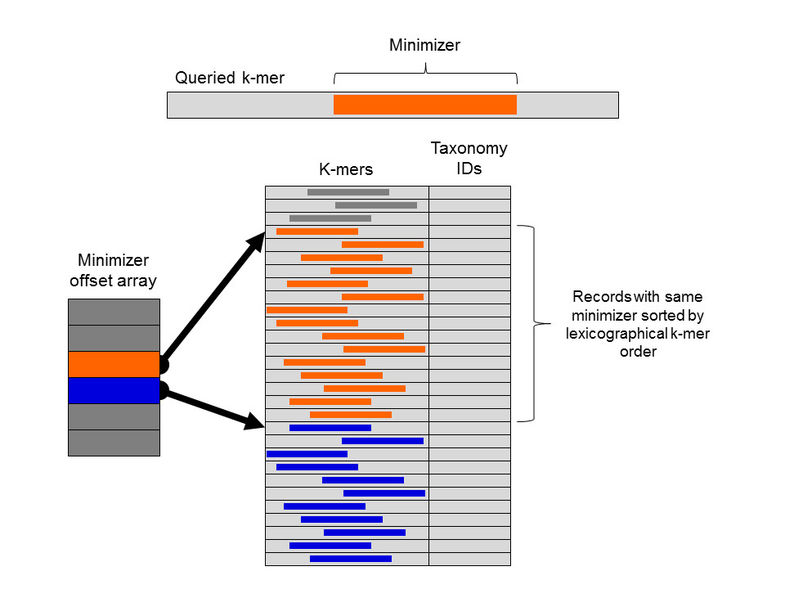
\includegraphics[width=\textwidth]{DbStructure.jpg}
	\caption{Prikaze strukture baze podataka (\cite{Kraken})}
	\label{BazaPodataka}
\end{figure}

Na slici 2.1 je prikazana struktura baze podataka koja se temelji na razvrstavanju i grupiranju podataka koji imaju istu \textit{minimizer} vrijednost. Tada se binarnim pretraživanje nalazi onaj spremnim u kojem se nalaze podaci s istom \textit{minimizer} vrijednošću kao i ulazni niz.
\\S ciljem poboljšanja brzine pretraživanja, uvodi se algoritam indeksiranja i raspoređivanja poznat pod imenom Minimizer (\cite{minim}). Računanje indeksa spremnika se odvija kroz dvije petlje. U prvoj petlji se iterira po broju spremnika te se za svaki od njih dohvaća njihov jedinstveni k-mer. Na osnovu njega se računa ključ te se popunjava niz brojem podataka koji ulaze u taj indeks. Nakon toga se računa pomak svih podataka te se zbrajaju s onim podacima koji se nalaze u nizu indeksa. Na kraju se iz varijable ofset kreira indeks vanjskom funkcijom.
 
\begin{figure}[hbp]
	\begin{algorithm}[H]
		\SetAlgorithmName{Algoritam}{algoritam}{List of algoritam}
		ptr <- pokazivač\_na\_k-mer\;
		k\_ct <- brojač kontejnera\;
		vrijednosti <- 1ull \footnote{\textit{Unsigned long long 1}} << (nt * 2)\;
		\While{brojač je različit od broja kontejnera}{
			brojač++\;
			dohvati\_k-mer(ptr)\;
			ključ <- izračunaj\_ključ()\;
			b\_brojač[ključ]++\;		
		}
		b\_pomak[vrijednosti +1]\;
		\For{i < vrijednosti}{
			b\_pomak = b\_pomak[i-1]+b\_brojač[i-1]\;
		}
		indeks(b\_pomak)\;
		\caption{Računanje indeksa spremnika (\cite{Kraken})}
		\label{Indeks}
	\end{algorithm}
\end{figure}

Algoritam 1 prikazuje načina računanja indeksa spremnika realiziran u izvornom kodu Kraken-a. Kroz petlju se dohvaćaju svi k-meri te se računaju ključevi za tablicu raspršenog adresiranja, te se povećava brojač koji označava koliko podataka se nalazi u jednom spremniku s jednim ključem. Tada se realizira pomak te se za vodi evidencija koliki je pomak potreban za svaki spremnik, tj. za koliko se mora pomaknuti pokazivač da bi došao do spremnika sa drugim ključem.
\\Prilikom sortiranja i indeksiranja se stvaraju svojevrsni spremnici u bazu podataka slijedno sadržavaju one podatke čiji k-meri imaju iste \textit{minimizer} vrijednosti. Podaci u svakom spremniku su leksikografski poredani kako bi se isti osposobio za daljnje binarno pretraživanje. Stvaranjem zasebnih spremnika se poboljšava pretraživanje na način da se za svaki ulazni podatak računaju njegovi k-meri te njegove \textit{minimizer} vrijednosti, te se pretragom liste indeksa dohvaća samo onaj spremnik koji sadrži istu \textit{minimizer} vrijednost. Prilikom dolaska novog podataka \textit{minimizer} vrijednost se ne računa odmah, nego se prvo vrši pretraga na spremniku na kojem smo već pozicionirani. Ako se podatak ne nalazi u zadanom spremniku, tada se prelazi na računanje \textit{minimizer} vrijednosti. Ako je \textit{minimizer} vrijednost ista kao i kod spremnika tada se podatak svrstava u neklasificirane te se svaka daljnja klasifikacija zaustavlja. U slučaju dobivanja \textit{minimizer} vrijednosti različite od trenutne pozicionira se na indeks izračunatog spremnika te se isti pretražuje. Način pretrage i podjele baze podataka prikazan je slici 2.1.



\section{Algoritam klasifikacije podataka}

Klasificiranje ulaznog podatka se odvija na više razina. Za početak se za ulazni genom računaju svi njegovi k-meri ( \textit{k} može biti zadan inicijalno ili ga korisnik može zadati). Zatim se za svaki k-mer kreiraju njegove \textit{LCA} vrijednosti, tj. traži se onaj podatak, u taksonomskom stablu, koji predstavlja prvog pretka tog k-mera. Od svih k-mera se tada kreira stablo koje predstavlja sve moguće klasifikacije za dani genom, a koje su dobivene upravo navedenim algoritmom. Svaka vrijednost u stablu ima izračunatu vrijednost koja predstavlja koliko k-mera se podudara sa tim podatkom. Te vrijednosti se nazivaju težinama čvora stabla. Ako za neki k-mer ne postoji poznati LCA , tada se on neće ni stavljati u navedeno stablo. Način rada koji uvodi težine za svaki čvor u stablu omogućuje veliku točnost u radu Krakena-a, tako da ako postoji neki put u stablu koji je pogrešan a težine su jako male, on će se zanemariti. Ako postoje dva puta u stablu koja imaju iste težine tada se samo za te podatke ponovno računa LCA te se pokušava odrediti koji put zapravo predstavlja točnu klasifikaciju. (\cite{Kraken})

\begin{figure}[!htbp]
	\centering
	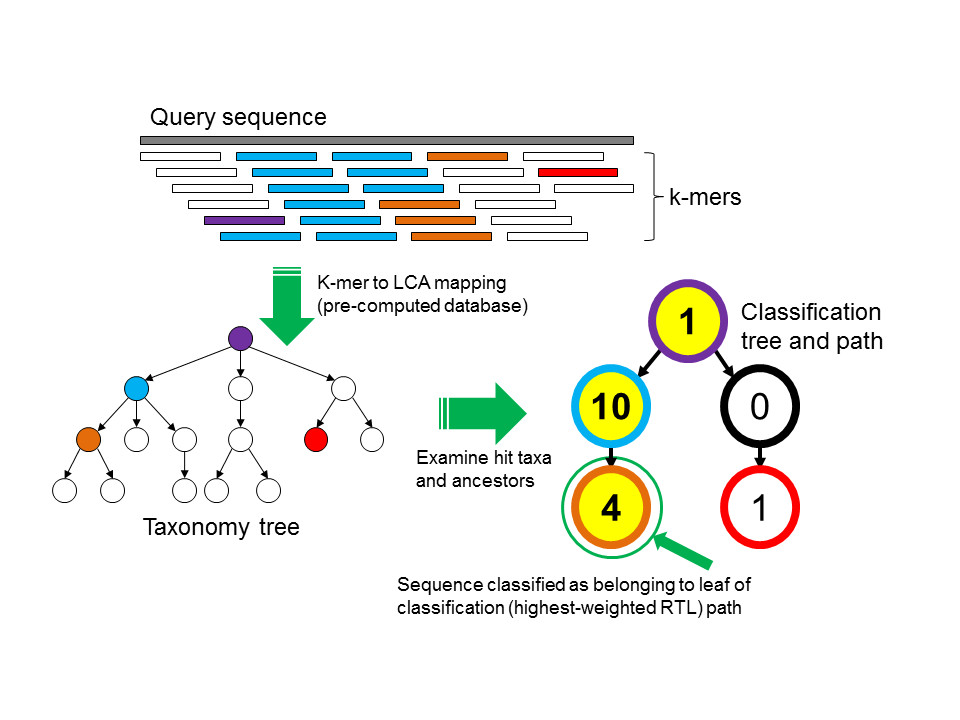
\includegraphics[width=\textwidth]{Work.jpg}
	\caption{Prikaz klasifikacije podataka (\cite{Kraken})}
	\label{Klasifikacija}
\end{figure}

Iz slike 2.2 se može vidjeti način rada algoritma. Nakon izračuna svih  k-mera ulaznog podatka, isti se pokušavaju klasificirati i izgraditi taksonomsko stablo pomoću vrijednosti najmanjeg zajedničkog pretka (LCA). To se izvodi pomoću predefinirane baze podataka. Upravo opisani dio rada prikazan je na slici 2.2  u gornjem dijelu slike. Nakon toga se računaju težine za svaki čvor u stablu. Težine predstavljaju broj k-mera koji se podudaraju sa tim istim čvorom. Težine su predstavljene na slici 2.2 u desnom kutu. Ako postoji više različitih puteva koji imaju iste težine, tada se za iste ponovno računa najmanji zajednički predak te se pokušava dokučiti koji je pravi put, tj. koji od čvorova je pravi predak između listova koje smo tražili. Nadalje ako postoji više puteva ali oni nisu istih težina, tada se put do zajedničkog pretka uzima onaj put koji ima najveću težinu, tj. kojem odgovara najviše k-mera. To je prikazano na slici 2.2 u desnom kutu, gdje možemo vidjeti da se od dva različita puta bira onaj lijevi upravo zbog toga jer je njegov zbroj težina veći od desnog. S time se zaključuje da su težine proporcionalne vjerojatnosti točnosti zadanog puta. (\cite{Kraken})


\section{LCA(\textit{Lower Common Ancestor})}
LCA(\textit{Lower common ancestor}) je jedan od osnovnih algoritamskih problema u strukturama stabala.A označava pronalazak čvora u stablu koji je najudaljeniji od korijena stabla, te je zajednički čvorovima \textit{u} i \textit{v}. Prvu ideju i definiciju LCA dali su Alfred Aho, John Hopcroft i Jeffrey Ullman 1973. godine u svom radu \textit{On finding lowest common ancestors in trees}. Zbog svoje složenosti te raznolike primjenjivosti ovaj problem je još uvijek aktualan, te se i danas objavljuje mnogo članaka i radova na tu temu. U uvodu svog rada autori navode glavni problem koji LCA pokušava riješiti. Problem se navodi kao primanje informacija o novim osobama u određenim vremenskim intervalima, te je pomoći zadanog algoritma potrebno točno odrediti sve veze između svakog novog čvora koji predstavlja danu informaciju. (\cite{lca1})
\begin{figure}[!htbp]
	\centering
	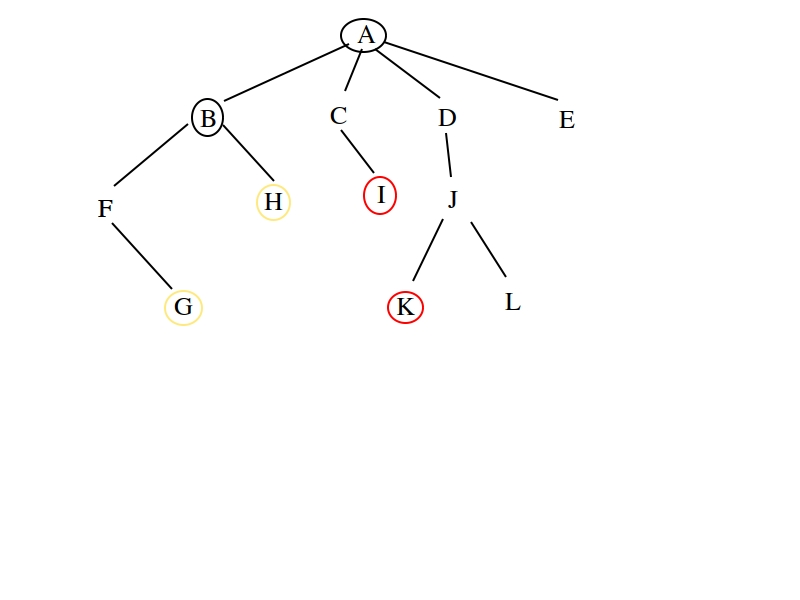
\includegraphics[width=\textwidth]{lca.jpg}
	\caption{Prikaz stabla i LCA vrijednosti}
	\label{LCA}
\end{figure}

Na slici 2.3 se nalazi prikaz strukture stabla te su bojama označeni listovi za koje želimo naći najmanjeg zajedničkog pretka (LCA). Crno obojeni čvorovi su čvorovi koji su preci tim dvama listovima. Tako je za listove H i G najmanji zajednički predak čvor B, dok je za listove I i K najmanji zajednički predak A. Ta ideja je predstavljena u radu \textit{On finding lowest common ancestors in trees} 1973. godine, te je predstavljen sljedeći pseudokod za određivanje najmanjeg zajedničkog pretka. (\cite{lca1,lca2,lca3})
\newline
\newline
\begin{algorithm}[H]
	
	\SetAlgorithmName{Algoritam}{algoritam}{List of algoritam}
	
	procedure getancestor(u,i):

	
		\If{ancestor(u,i-1) = undefined then;}{
			ancestor(u,i) <- getancestor(getancestor(u,i-1),i-1)\;
		}
		resultis ancestor(u,i)\;
	\caption{Dohvaćanje pretka zadanog čvora \cite{lca1}}
	\label{LCA algoritam 1}
\end{algorithm}

Algoritam 2 predstavlja metodu getancestor(u,i), koja prima čvor \textit{u} te dubinu \textit{i}. Funkcija dohvaća pretka koji je na $2^i$-toj poziciji te ga stavlja u niz koji sadrži pretke zadanog čvora. \textit{Getancestor} se poziva tijekom traženja najmanjeg zajedničkog pretka. Ova metoda predstavlja očuvanje svih informacija o precima za jedan čvor. 
\newline
\begin{algorithm}[H]

	\SetAlgorithmName{Algoritam}{algoritam}{List of algoritam}
		procedure find(u,v,i,d):\\
		\eIf{i = 0}{
			resultis ancestor(u,0)\;
		}{
			\eIf{getancestor(u,i-1)=getancestor(v,i-1)}{
				resultis find(u,v,i-1,d)\;
			}{
				resultis find(getancestor(u,i-1),getancestor(v,i-1),min(i-1,|\_log(d-$2^{(i-1)}$)\_|),d-$2^{(i-1)}$)\;
			}
		}
	\caption{Pronalazak najmanjeg zajedničkog pretka između dva čvora (\cite{lca1})}
	\label{LCA algorithm 2}
	
\end{algorithm}

Algoritam 3 predstavlja metodu koja pronalazi najmanjeg zajedničkog pretka za ulazne podatke \textit{u} i \textit{v} koji su na dubini \textit{d}. Početne pretpostavke su da je \textit{d} > $2^{(i-1)}$ te su im $2^i$-ti preci jednaki ili ne postoje. Zadana metoda radi na način da u svakom novom koraku smanjuje radni prostor koji pretražuje , tako da je put do najmanjeg zajedničkog pretka uvijek u zadanom prostoru. Gore navedene dvije metode omogućuju stvaranje metode koja osigurava pronalazak najmanjeg zajedničkog pretka uz pravilno biranje početnih uvjeta. Budući da se zadnji uvijek računa logaritamskom funkcijom, algoritam je optimiziran tako da se podaci predstavljaju kao binarne znamenke, te se u svakom koraku petlje pomiče za jedan bit dok ne dođe do kraja.
\chapter{Algoritmi indeksiranja i pretrage}
\section{Minimizer - algoritam za reduciranje podataka}
Usporedba podataka je osnova moderne bioinformatike. Ona se danas temelji na metodi \textit{seed-and-extend} (pronađi uzorak). Za svaki ulazni podatak se uzima samo jedan uzorak, te se on uspoređuje u bazi podataka. Ako se nađe poklapanje tada se taj uzorak proširuje na cijeli podatak te se ponovno uspoređuje. Da bi sve to funkcioniralo potrebno je uzeti uzorak za svaki podskup u jednom genomu, što , za kompleksnije genome, zauzima jako puno memorije.Na ideju rješenja su došli Michael Roberts, Wayne Hayes, Brian R. Hunt, Stephen M. Mount i James A. York u svom radu \textit{Reducing storage requirements for biological sequence comparison} (\cite{minim}). Koristi se isti način rada, tj.\textit{seed-and-extend}, uz razliku da se ne uzimaju svi uzorci, nego samo mali podskup jedinstvenih, nazvanih \textit{minimizer-i}.(\cite{minim})
\\ Navedeni algoritam sažimanja se koristi i u Kraken bazi podataka, te ju uvelike smanjuje i pospješuje brzinu izvođenja. Prilikom kreiranja MiniKraken baze podataka se koristi isti način rada, uz razliku da se odbacuje samo određeni postotak prvih i zadnjih vrijednosti. Da bi spremnici u kojima su sadržani podaci s istim \textit{minimizer} vrijednostima zadržao svojstvo kolekcije, potrebno je da su ti isti podaci normalno distribuirani, što se postiže brisanjem pola bitova prilikom ispitivanja jednakosti. S ciljem pospješenja brzine izvođenja, jer svako računanje \textit{minimizer} vrijednosti je relativno skupo, prilikom klasifikacije podatka koristi se onaj spremnik koji je korišten prije, te ako k-meri nisu nađeni u njemu, računa se \textit{minimizer} vrijednost. Ako je \textit{minimizer} vrijednost jednaka kao u spremniku zaključuje se da se podatak ne može klasificirati, inače se pozicionira u dani spremnik te se ponovno vrši pretraga. (\cite{Kraken})

Postoje dvije vrste \textit{minimizer} vrijednosti: unutarnje i vanjske. Svakoj od njih je srž računanja isti, tj. za ulazni niz se računaju svi njegovi k-meri za zadani k, te se iz njih tada bira onaj k-mer koji je leksikografski najmanji. 

\begin{figure}[htbp]
	\centering
	
	\begin{tabular}{l|l|llllllll|}
		\multicolumn{2}{l|}{Pozicija:}                                                                                       &  & 1 & 2 & 3 & 4          & 5          & 6          & 7 \\ \hline
		\multicolumn{2}{l|}{Ulazni niz:}                                                                                     &  & 2 & 3 & 1 & 0          & 3          & 4          & 3 \\ \hline
		\multicolumn{2}{l|}{\multirow{5}{*}{\begin{tabular}[c]{@{}l@{}}k-meri\\ s\\ podebljanim\\ minimizerom\end{tabular}}} &  & 2 & 3 & 1 &            &            &            &   \\
		\multicolumn{2}{l|}{}                                                                                                &  &   & 3 & 1 & 0          &            &            &   \\
		\multicolumn{2}{l|}{}                                                                                                &  &   &   & 1 & 0          & 3          &            &   \\
		\multicolumn{2}{l|}{}                                                                                                &  &   &   &   & \textbf{0} & \textbf{3} & \textbf{4} &   \\
		\multicolumn{2}{l|}{}                                                                                                &  &   &   &   &            & 3          & 4          & 3 \\ \hline
	\end{tabular}
	\caption{K-meri ulaznog niza s minimizer-om (\cite{minim})}
	\label{Minimizer}
\end{figure}

Slika 3.1 prikazuje način odabira \textit{minimizera} za ulazni niz. Ulazni niz je podijeljen na 3-mere , a za računanje \textit{minimizer-a} se koristi prozor od 5 k-mera. Korištenje prozora znači da se samo u 5 k-mera odjednom traži \textit{minimizer} vrijednost. Budući da je \textit{034} leksikografski najmanji podniz on se uzima kao zadani \textit{minimizer}. Algoritam \textit{minimizer} nam garantira da će dva niza koja su ista sadržavati barem jednu istu \textit{minimizer} vrijednost.
\section{Binarno pretraživanje}
Za pretraživanje svakog spremnika se koristi binarno pretraživanje. Binarno pretraživanje je jedan od osnovnih algoritama u računalnoj znanosti. Glavni zadatak algoritma je pronalazak vrijednosti u sortiranom nizu. Osnovna i glavna pretpostavka jest da je niz sortiran, u suprotnom sam algoritam nema smisla.
\newline
\newline
\begin{algorithm}[H]
	\SetAlgorithmName{Algoritam}{algoritam}{List of algoritam}
	binarno\_pretraživanje(niz,cilj):\\
	lo = 1, hi = size(niz)\;
	\While{lo <= hi}{
		mid = lo + (hi - lo) / 2\;
		\eIf{niz[mid] == cilj}{
			return mid\;
		}{
			\eIf{niz[mid] < cilj}{
				lo = mid + 1\;	
			}{
				hi = mid + 1\;
			}
		}
	}
	\caption{Binarno pretraživanje}
	\label{BinarnoP}
\end{algorithm}

Inicijalno je radni prostor binarnog pretraživanja cijeli ulazni niz. Tada se pozicionira na sredinu tog niza, te se ispituje je li vrijednost na sredini jednaka onoj koju mi tražimo. Ako je rezultat potvrdan izlazimo iz petlje te vraćamo poziciju te vrijednosti. U protivnom se ispituje odnos tražene vrijednosti i one koja je na sredini. Ako je vrijednost na sredini manja od tražene radni prostor postavljamo na onu polovicu koja se nalazi desno od indeksa, tj. prelazimo u  polovicu koja sadrži veće vrijednosti, u suprotnom se pozicioniramo na manju polovicu. Složenost binarnog pretraživanja je O(logN), gdje je N broj znakova u nizu. Logaritam je sporo rastuća funkcija, stoga je binarno pretraživanje jako efikasan algoritam. Kao primjer za pretragu imenika od milijun imena, pomoću binarnog pretraživanja bismo pronašli traženu vrijednost u najviše 21 korak.


\chapter{Pseudokod i razrada algoritma}
Rješenja navedenog problema o korištenju baze podataka na ograničenim resursima se sastoji iz nekoliko dijelova. Za početak je potrebno podijeliti bazu podataka na manje cjeline, zatim je potrebno ostvariti straničenje na tim cjelinama.
\section{Problemi kod korištenja Kraken baze podataka}

Iako je prvotna ideja bila koristiti Kraken bazu podataka, te je algoritam i osmišljen upravo za nju, zbog tehničkih problema se moralo odustati od te ideje. Pod tehničke probleme misli se na nemogućnost pristupa bazi podataka, a bez pristupa se nije mogao provesti nijedan algoritam nad njom. Sama baza podataka je u nepodržanom formatu za bilo koji preglednik baze podataka koji sam uspio naći, a proučavanjem izvornog koda Kraken alata se nije moglo puno zaključiti. Kod je slabo zakomentiran te je veliki problem snaći se u takvom okruženju. Stoga se za daljnji rad koristi jednostavna baza podataka od par stotina kilobyte-a.(\cite{Database})

\section{Podjela baze podataka}
Iz gore navedenih razloga odlučeno je prezentirati rad algoritma, te samu raspodjelu baze podataka na uzorku baze podataka. (\cite{Database})
\begin{figure}[!htbp]
	\centering
	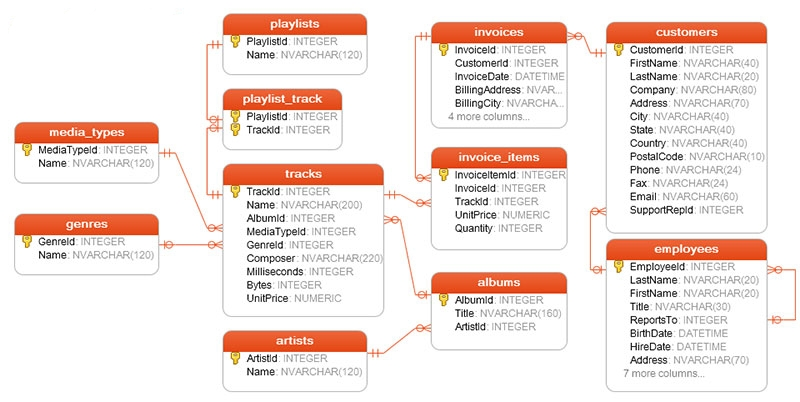
\includegraphics[width=\textwidth]{sqlite-sample-database-color.jpg}
	\caption{Prikaz korištene baze podataka (\cite{Database})}
	\label{Db}
\end{figure}
Baza podataka je sqlite3 tipa, te se u izvornom kodu programa koristi paket sqlite3.\\
Podjela baze podataka na cjeline je ostvarena bash skriptom, koja  pomoću sqlite3 naredbi iz zadane baze podataka kreira datoteku koja sadrži sql naredbe koje stvaraju kostur baze podataka, tj. stvara zadani broj (trenutno je to 5 baza podataka) identičnih baza podataka kao originalna ali bez ijednog podatka u sebi.\\ Budući da je već gotovu bazu podataka gotovo nemoguće podijeliti na funkcionalne baze, morao se koristiti pristup gdje se ista pretvara u niz sql upita.

\begin{algorithm}[H]
	\SetAlgorithmName{Algoritam}{algoritam}{List of algoritam}
		\If{postoji schema.sql}{izbriši schema.sql\;}
		\If{postoji dump.sql}{izbriši dump.sql\;}
		sqlite3 imebaze .schenm -> schema.sql\;
		sqlite3 imebaze .dump -> dump.sql\;
	\caption{Podjela baze podataka}
	\label{PodjelaBp}
\end{algorithm}

Gore navedenim dijelom koda se stvaraju datoteke schema.sql i dump.sql. Schema.sql sadrži SQL naredbe koji stvaraju strukturu originalne baze podataka, a dump.sql se sastoji od SQL naredbi koji pune bazu podataka podacima iz originalne baze podataka.
\\Budući da želimo bazu podataka podijeliti na cjeline potrebno je datoteku dump.sql podijeliti na onoliko datoteka koliko želimo da imamo baza podataka. U svrhe demonstracije rješenja dump.sql je podijeljen u 5 cjelina koje su slijedno razdvojene. \\Za Kraken bazu podataka se može koristiti datoteka koja sadrži indekse svakog spremnika, te možemo dobiti baze podataka koje sadrže samo one podatke čiji k-meri imaju jednake minimizer vrijednosti. Iza tog problema se krije ne jako zahtjevna logika koju relativno lako možemo realizirati u bash skripti.
\\Time ne završava podjela baze podataka na manje dijelove, naime potrebno je kreirati svaku bazu podataka te unijeti podatke u svaku zasebno. Iz dump.sql datoteke je dobiveno 6 dump.split.000x.sql datoteka , koje će svaka za sebe graditi bazu podataka. Kako smo datoteku podijelili pomoću jednostavne \textit{split} naredbe u bash-u dobivene datoteke nisu pravilno konfigurirane za kreiranje. Stoga je potrebno , ako ne postoji, na početku svake datoteke upisati SQL naredbu  \textit{BEGIN TRANSACTION}, te na kraju iste , opet ako ne postoji, upisati naredbu \textit{COMMIT}. To je izvedeno sljedećim dijelom bash skripte.

\begin{algorithm}[H]
	\SetAlgorithmName{Algoritam}{algoritam}{List of algoritam}
	\For{svaku datoteku u direktoriju}{
		\If{"BEGIN TRANSACTION" se ne nalazi na početku datoteke}{
			dodaj\_BEGIN\_TRANSACTION\_na\_početak\;
		}
		\If{"COMMIT" se ne nalazi na kraju datoteke}{
			dodaj\_COMMIT\_na\_kraj\;
		}
	}
	\caption{Osposobljavanje dump datoteka}
	\label{DumpBp}
\end{algorithm}

Naposljetku je potrebno kreirati bazu podataka. To se radi na način da se za svaku dump.split.000x.sql datoteku kreira baza podataka koja sadrži samo kostur originalne baze, te se u nju tada pomoću navedene datoteke ubacuju podaci. Na kraju izvedbe zadanog programa smo dobili 6 baza podataka koje zajedno imaju sve podatke koje je zadržavala originalna baza podataka.

\section{Straničenje}
Za prezentaciju algoritma straničenja koristit će se jednostavni SQL upit koji želi dohvatiti sve podatke za neku tablicu. Algoritam straničenja je prvotno bio osmišljen u verziji koja bi bila dosta brža, ali za ovaj rad je obrađeno samo standardno straničenje.

	\begin{algorithm}[H]
		\SetAlgorithmName{Algoritam}{algoritam}{List of algoritam}
		\For{ima podataka u listi}{
			\For{i < broj\_baza\_podataka}{
				otvori bazu podataka()\;
				pozovi SQL upit nad bazom podataka()\;
				zatvori bazu podataka()\;	
			}
		}
		\caption{Algoritam straničenja}
		\label{Stranicenje}
	\end{algorithm}

Gore navedeni pseudokod predstavlja algoritam koji je implementiran za potrebe ovoga rada. Poboljšana verzija bi se sastojala od toga da se za ulazni podataka izračuna indeks te se otvori i pretraži samo baza podataka koja može sadržavati zadani indeks. Taj algoritam je predstavljen sljedećim pseudokodom.
\newline
	\begin{algorithm}[H]
		\SetAlgorithmName{Algoritam}{algoritam}{List of algoritam}
		\For{ima podataka u listi}{
			izračunaj indeks za ulazni podatak();
			\eIf{otvorena baza je istog indeksa ko podatak}{
				pozovi SQL upit nad bazom podataka()\;
			}{
				
				zatvori bazu podataka()\;
				pozovi SQL upit nad bazom podataka()\;
				otvori bazu podataka()\;
			}
		}
		\caption{Poboljšani algoritam straničenja}
		\label{Stranicenje2}
	\end{algorithm}

Svi podaci su ostali sačuvani, te je za tablicu imena \textit{albums}, SQL upitom SELECT * FROM albums rezultat prikazao sve podatke koji se nalaze u originalnoj bazi.
\chapter{Analiza učinkovitosti rješenja}
Zbog nemogućnosti korištenja Kraken i MiniKraken baze podataka testovi koje je moguće provesti za zadani algoritam su ograničeni. Prvi provedeni test je izveden naredbom SELECT * FROM playlists te je utvrđeno da su svi podaci ostali sačuvani, te da \textit{callback} metoda, koja je zaslužena za ispisivanje svih dobivenih podataka, nema nikakvih problema s njihovom interpretacijom. 
\newline
\begin{figure}[hbp]
	\begin{lstlisting}
static int callback(void *data, int argc, char **argv,char **azColName){
	int i;
	fprintf(stderr, "%s:", (const char*)data);
	for(i=0; i<argc; i++){
		printf("%s=%s\n", azColName[i],argv[i] ? argv[i] : "NULL");
	}
	printf("\n");
	return 0;
}
	\end{lstlisting}
\end{figure}

Algoritam 8 predstavlja funkciju koja za prima rezultat sql naredbe te ga parsira u format koji je prikladan za čitanje.
\\S obzirom na vrijeme izvođenja u samom početku se moglo zaključiti da će program raditi sporije, pogotovo na većim bazama koje će se morati učitati u RAM. Međutim cilj ovog rješenja je osposobljavanje na rad, ali i spremnost na nešto sporiji rad. Naravno sve se još da optimizirati korištenjem indeksa za interpretaciju i dohvaćanje raznih baza podataka. Jedan od glavnih problema ovog pristupa je bio kako uspješno već gotovu bazu podataka raspodijeliti u manje a da podaci ostanu kontinuirani i indeksi u svim tablicama ostanu očuvani, što je uspješno odrađeno. Iako neobičan, pristup problemu tako da se cijela baza podataka pretvori u niz SQL upita se pokazao kao jako dobar, te će se zasigurno koristiti u mom daljnjem istraživanju i pokušavanju rješenja navedenog problema. Budući da je baza podataka jako mala nije se mogao provesti smislen test potrošnje vremena koji će potkrijepiti gore navedenu teoriju.
\section{Za budućnost}
U budućem radu ću se više osloniti na implementaciju rješenja konkretno na Kraken bazu podataka, koja je do sada predstavljala veliki problem. Pokušat kontaktirati autore samog alata se u dogovoru s njim raditi na rješavanju, po mom mišljenju, jednog jako zanimljivog problema koji može poboljšati Kraken . Budući rad podrazumijeva dolaženje do podataka koji se nalaze u Kraken bazi podataka, te podjela iste baze na manje cjeline. Razlika od dosadašnjeg rada je da se baza podataka neće dijeliti na bilo koje cjeline, nego će jednu novu bazu podataka činiti jedan spremnik jedinstvenog \textit{minimizera}. Tada u izradu nastupa implementiranje straničenja podataka te poboljšanje samog straničenja korištenjem liste indeksa.
\chapter{Zaključak}
Bioinformatika je interdisciplinarna znanost koja spaja više prirodno-matematičkih znanosti. U zadnjim desetljećima je doživjela veliki porast. Upravo zbog svog razvitka se razvila potreba za programima koji mogu jako brzo i precizno klasificirati ulazni metagenom. Jedan od takvih programa je i Kraken. Svojom izrazitom preciznošću i brzinom izvođenja u vrhu je alata da  klasificiranje genoma, i zbog toga je odabran za analizu u ovom radu. Uspješno spaja nekoliko algoritama za indeksiranje, pretragu te klasifikaciju podataka. Za klasificiranje podataka se koristi LCA algoritam, te za indeksiranje i pretragu baze podataka se koristi minimizer algoritam. Problem kojim se bavi ovaj rad se odnosi upravo na bazu podataka koja je prevelika za učitavanje u RAM na većini osobnih računala. \\Kako bazu od nekoliko desetak GB ubaciti u RAM koji je samo nekoliko GB? \\Idejom raspodjele baze podataka te straničenjem tih baza se pokušalo približiti rješenju, te se ovim radom to i uspjelo. Iako se poboljšao utrošak memorije, vremenska složenost pretrage je porasla, što je bilo očekivano. Rana testiranja, koja se nisu uspjela odviti na Kraken bazi podataka, su pokazala jednu od najbitnijih značajki koja se morala zadržati, a to je očuvanje svih podataka i njihovih indeksa, te jednakost rezultata pretrage na originalnoj bazi podataka i manjim bazama. U daljnjem radu na ovom problemu pokušat će se sve to implementirati na prvotno namijenjenu bazu podataka te ispitati ponašanje u tom slučaju.

\bibliography{literatura}
\bibliographystyle{fer}


\begin{sazetak}
Straničenje velike baze podataka se odvija u dva koraka. Prvi je podjela baze podataka na manje cjeline( baze podataka manjeg memorijskog kapaciteta). On je ostvaren pomoću bash skripte koja, uz sqlite3 naredbe, uspijeva napraviti kostur originalne baze te SQL upite za punjenje baze podacima.\\
Drugi  korak je samo straničenje koje se iterira po svim bazama te traži podatak koji želimo obraditi. Za nastavak i poboljšanje straničenja se može uvesti lista indeksa baza podataka te se jednostavnim pretraživanjem liste može utvrditi samo jedna baza podataka koju trebamo učitati.

\kljucnerijeci{straničenje, baza podataka, Kraken, metagenom, k-mer, LCA, minimizer}
\end{sazetak}

% TODO: Navedite naslov na engleskom jeziku.
\engtitle{Algorithm for Paging Large-Scale Genome Database}
\begin{abstract}
Paging of a large-scale database is made from two steps. The first one is splitting a database into smaller units( databases that contains less memory). It is done by the bash script that manages to create skeleton of original database, and to fill the databases with data.
\\The second step is paging itself that iterates over all databases and searches the data that we want to process. For of paging one can use index list and, by simple search of that list, can determine only one database that needs to be loaded	.

\keywords{paging, database, Kraken, metagenom, k-mer, LCA, minimizer}
\end{abstract}

\begin{appendices}
	\chapter{Upute za korištenje programske potpore}
	Upute za korištenje programske potpore:
	\begin{description}
		\item[1.] Za koristiti programsku podršku potrebno je raditi na nekoj od Linux distribucija, te ista mora sadržavati instalirane sqlite3 i sqlite3-devel pakete.
		\item[2.] Za koristiti programsku podršku potrebno je raditi na nekoj od Linux distribucija, te ista mora sadržavati instalirane sqlite3 i sqlite3-devel pakete.
		\item[3.] Za rad sa izvršnim programom preuzeti direktorij koji sadrži sve zadane komponente.
		\item[4.] Pozicionirati se u direktorij Database.
		\item[5.] Pokrenuti skriptu splitScript.sh sa argumentima imena baze podataka te brojem baza koje želimo napraviti.
		\item[6.] Dump.sql i schema.sql će biti spremljeni u trenutni direktorij.
		\item[7.] Baze podataka će biti spremljene u direktorij Databases dok će raspodijeljena dump datoteka biti u Splitted direktoriju.
		\item[8.] Pokrenuti Makefile.
		\item[9.] Pokrenuti izvršni program sa argumentom broja baza koje želimo koristiti.
	\end{description}
\end{appendices}

\end{document}
